\documentclass{article}
\usepackage{graphicx} % Required for inserting images
\usepackage{CJKutf8}
\usepackage{amsthm}
\usepackage{mdframed}
\usepackage{float}

% 自定義 "Definition" 環境
\newmdtheoremenv{definition}{Definition}

\title{hw8}
\author{110201534 楊成偉}
\date{}

\begin{document}
\begin{CJK*}{UTF8}{bkai}
\maketitle

\section*{step1}
we will show the following graph satisfing the statement.
\begin{figure}[H]
    \centering
    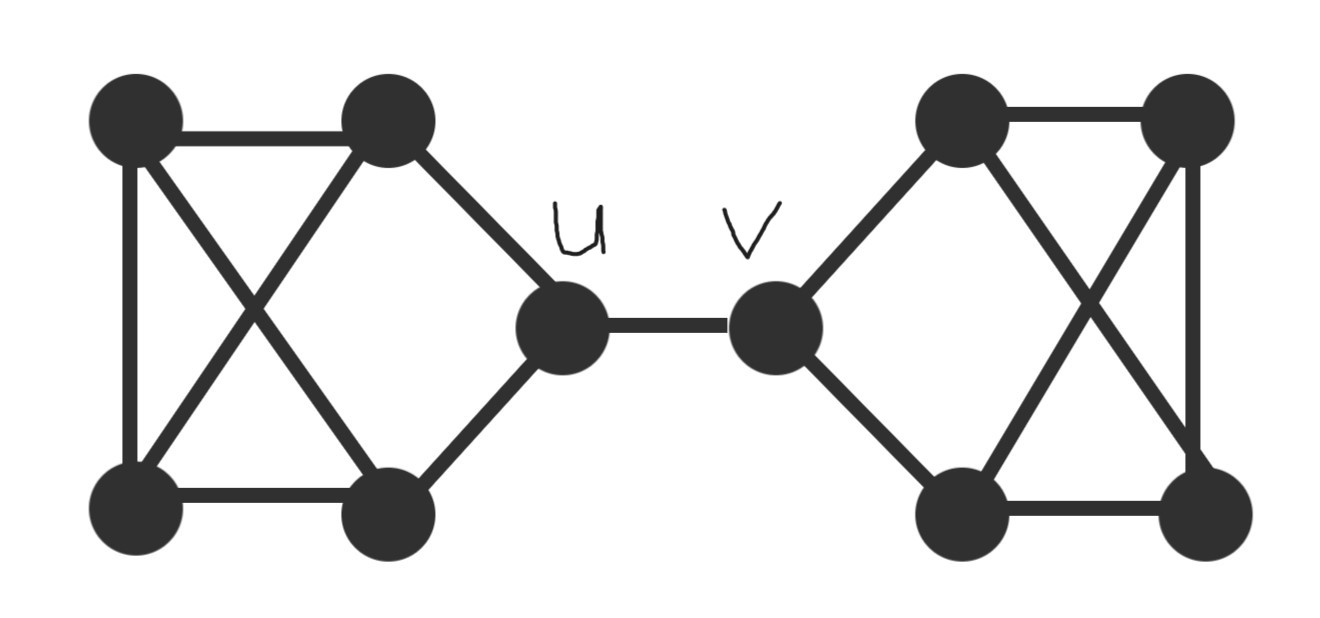
\includegraphics[scale = 0.1]{hw8g.jpg}
    \caption{A simple 3-regular graph with connectivity 1}
\end{figure}
since if we remove the vertex u, then the graph will be disconnected. so K(G) = 1 and if we remove the edge uv, G-uv also be disconnected, so k'(G) = 1.
\section*{step2}
it is obvious that uv is a cut-edge, and the number of the componets in G-e is 2.
\section*{step3}
In the two componets in G-e, the degree of u (in $H_{1}$)and v (in $H_{2}$) is 2, and the degredd of other vertice is 3.
\section*{step4}
we know that sum of degree for all vertice in G is even, if we remove the edge uv, the value also is even, since the two componets in G-uv is isomophism. so we can only discuss in $H_{1}$. In $H_{1}$, 
\section*{step5}

\section*{step6}

\section*{conclusion}

\end{CJK*}
\end{document}
